\subsection{Lösungsansatz: Prediktive Kodierung}
Wie daten verloren gehen, warum 

\subsubsection{Variante: einfaches Subsampling}
Für die erste Variante wird das Subsampling des DCT-Lösungsansatzes verwendet. Es reduziert die Punktmenge auf die Anzahl des Ist-Zustands. Die Feldlinien werden mit einer PCA in ein lokales Koordinatensystem transformiert. Im lokalen System können die Koordinaten mit 16 Bit Genauigkeit dargestellt werden. 16 Bit im Koordinatensystem der Sonne reichen nicht aus und führen zu einem grösseren Fehler als der Ist-Zustand.\\
In dieser Variante wird der Einfluss von vier Prediktoren getestet ($x$ sind die Bekannten Punkte und $y$ die Vorhersage):
\begin{itemize}
\item Konstanter Prediktor: Nimmt an, dass der nächste Wert im Kanal gleich dem  letzten Wert ist ($x = y$).
\item Linearer Prediktor: Nimmt an, dass die Steigung die Steigung zum nächsten Wert konstant bleibt ($x_1+(-x_2+x_1) = y$).
\item Linearer Prediktor mit Moving Average: Nimmt die durchschnittliche Steigung der letzten Werte.
\item Adaptiver Linearer Prediktor mit Moving Average: Berücksichtigt den Fehler der letzten Vorhersage.
\end{itemize}

\begin{figure}[!htbp]
	\center
	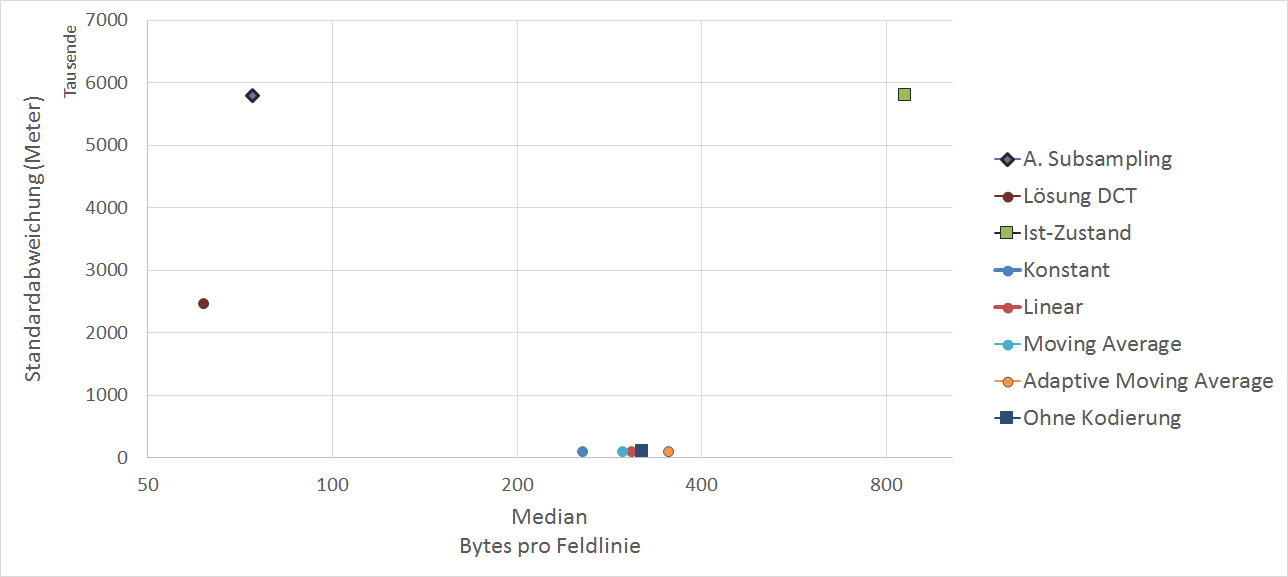
\includegraphics[width=1\textwidth,keepaspectratio]{./pictures/resultate/loesung2/variante0/resultate.png}
	\caption{Kompressionsraten der vier Prediktoren im Vergleich zum Ist-Zustand.}
	\label{resultate:loesung2:simple:resultate}
\end{figure}
Im Diagramm der Abbildung \ref{resultate:loesung2:simple:resultate} sind die Kompressionsraten der jeweiligen Prediktoren dargestellt. Ein Diagramm mit der PSNR-HVS-M wurde nicht erstellt. Sie ist für alle Prediktoren gleich und liegt bei $140.7$ dB. Unerwartet ist, dass der Konstante Prediktor mit $255$ Bytes pro Feldlinie die beste Kompression erreichte, obwohl die Daten nicht zuverlässig vorhersagen kann. Im Vergleich mit dem Moving Average Prediktor sind die Fehler der Vorhersagen 
bis zu $5$ Mal grösser, verbrauchen aber $40$ Bytes weniger um eine Feldlinie abzuspeichern. Der Fehler bleibt jedoch Konstant. Eine Möglichkeit ist, dass die Rar Kodierung sich wiederholende Muster findet.\\
Eine mögliche Optimierung ist die Adaptive Byte Kodierung der DCT-Variante, beschrieben im Abschnitt \ref{konzept:loesung1:kodierung}. Das Diagramm der Abbildung \ref{resultate:loesung2:simple:resultate_byte} zeigt die Resultate mit der Byte Kodierung. Der Konstante Prediktor verbraucht mit der Adaptiven Kodierung mehr Speicherplatz. Die Kompressionsrate der anderen Prediktoren wird durch die Adaptive Kodierung deutlich verbessert. Der Lineare Prediktor erreicht mit $214$ Bytes pro Feldlinie die beste Kompression. Das bedeutet, dass die Fehler des Konstanten Prediktors grösser sind, als die der anderen Prediktoren. Es bestätigt die Vermutung, dass die anderen Prediktoren die Daten besser vorhersagen können. Die Kompressionsrate des Konstanten Prediktors ist auf die Rar Kodierung zurückzuführen, welche in den Prediktor-Fehler Muster erkennen und effizient kodieren kann.\\ 
\begin{figure}[!htbp]
	\center
	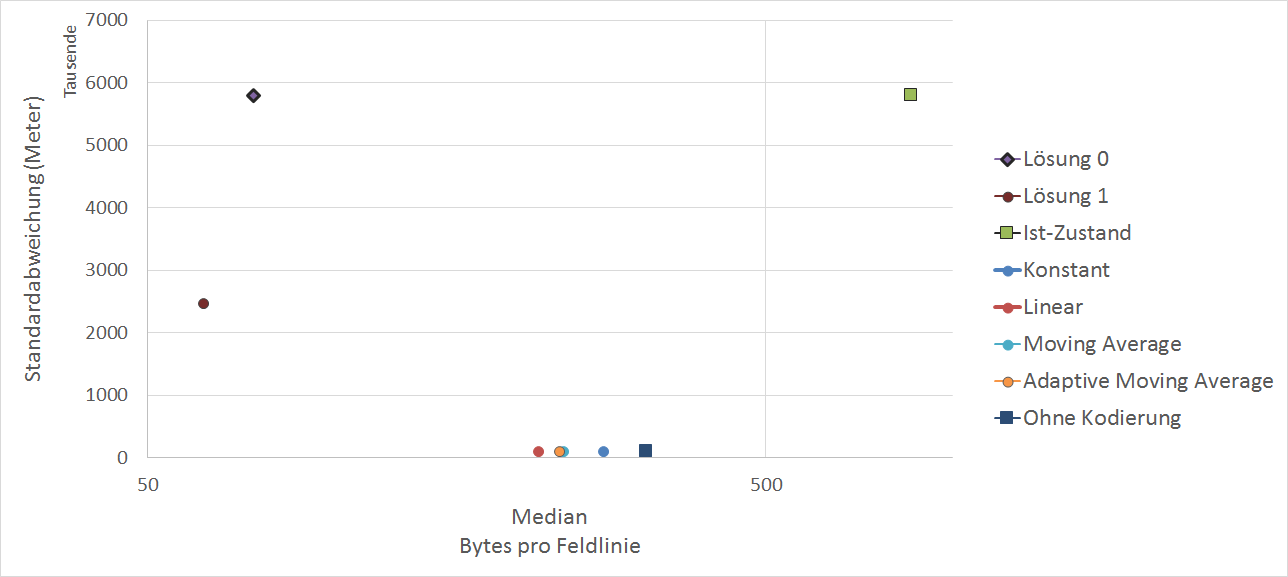
\includegraphics[width=1\textwidth,keepaspectratio]{./pictures/resultate/loesung2/variante0/resultate_byte.png}
	\caption{Kompressionsraten der Prediktoren mit Adaptiver Byte Kodierung.}
	\label{resultate:loesung2:simple:resultate_byte}
\end{figure}
Der Linare Prediktor kann eine Feldinie mit etwa $214$ Bytes darstellen, was eine Kompressionsrate von $4$ ergibt.

\subsubsection{Variante: Adaptives Subsampling}
Um mit diesem Ansatz in die selbe Grössenordnung zu gelangen wie die Lösungsansätze Adaptives Subsampling und DCT müssen mehr Informationen gelöscht werden. Es werden andere Parameter verwendet und im Schnitt $50\%$ mehr Punkte übertragen als im Lösungsansatz des Adaptiven Subsampling.
\begin{figure}[!htbp]
	\center
	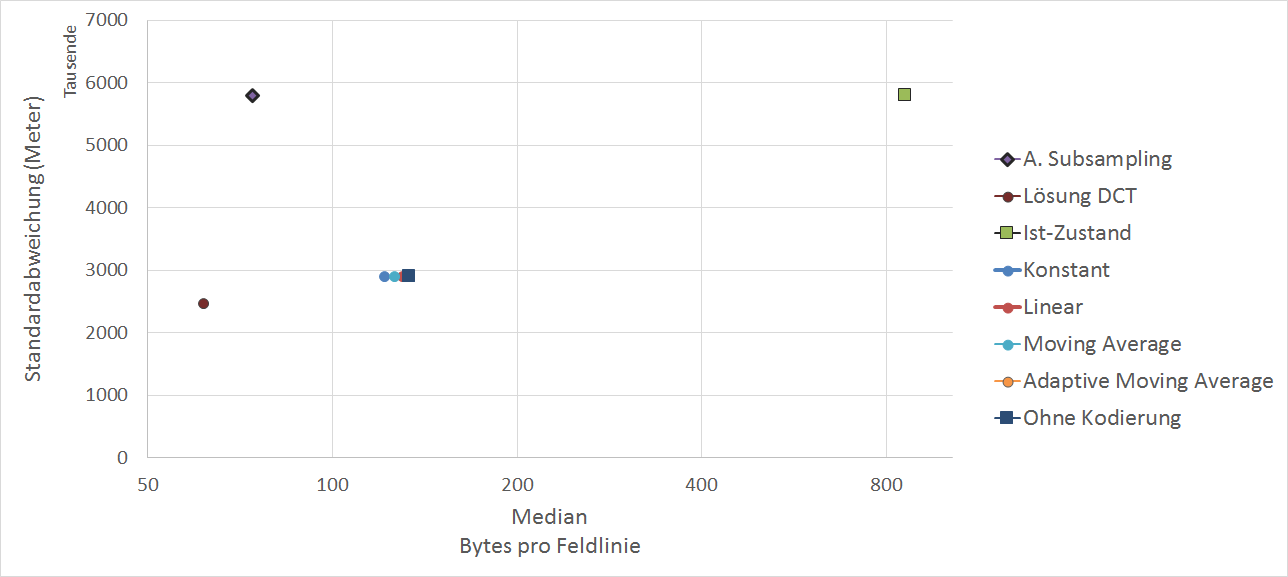
\includegraphics[width=1\textwidth,keepaspectratio]{./pictures/resultate/loesung2/variante1/resultate_euler.png}
	\caption{Kompressionsraten der Prediktiven Kodierungen mit dem adaptiven Subsampling.}
	\label{resultate:loesung2:adaptive:euler}
\end{figure}
Das Diagramm der Abbildung \ref{resultate:loesung2:adaptive:euler} zeigt die Kompressionsraten. Die Resultate liegen dicht beieinander und der Abstand zwischen Kodierung und der Kompression, welche ohne Kodierung erreicht wird wurde drastisch vermindert. Die Kodierungen erreichen eine PSNR-HVS-M von $139,2$. Dies liegt an den Eigenschaften des Outputs vom Angle Subsampling: Die Kanäle einer Feldlinie sind nach dem Subsampling weniger stetig. Der Lineare Prediktor ist bei diesen Daten nicht besser als keine Kodierung.

Um die Vorhersage zu verbessern werden die Punkte in das sphärische Koordinatensystem transformiert. Mit dieser Transformation und dem Angle-Subsampling werden sich stetigere Kanäle erhofft.
\begin{figure}[!htbp]
	\center
	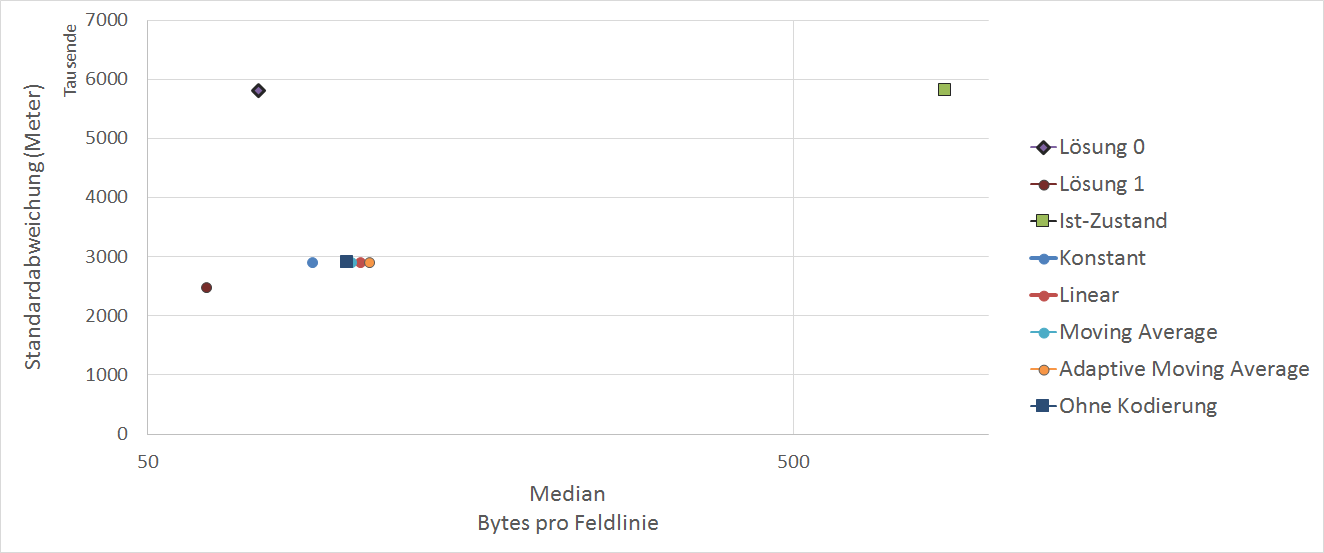
\includegraphics[width=1\textwidth,keepaspectratio]{./pictures/resultate/loesung2/variante1/resultate_spherical.png}
	\caption{Kompressionsraten der Prediktiven Kodierungen mit im sphärischen Koordinatensystem.}
	\label{resultate:loesung2:adaptive:spherial}
\end{figure}
Die Kompressionsraten der Kodierungen im sphärischen Koordinatensystem sind im Diagramm der Abbildung \ref{resultate:loesung2:adaptive:spherial} dargestellt. Die Phänomene im Diagramm der Abbildung \ref{resultate:loesung2:adaptive:euler} wurden weiter verstärkt, die Kodierungen erbringen keine Verbesserung mit Ausnahme der konstanten Kodierung. Durch die Verwendung des sphärischen Koordinatensystems wird eine bessere Kompression erreicht, da die PCA-Koeffizienten gespart werden können.

\subsubsection{Median Prediktive Kodierung}
Allgemeine Kurven kodieren, beschrieben im Abschnitt \ref{konzept:prediktiv}. Zusätzliche Quantisierung eingebaut.
figure
figure psnr-hvs-m
Deutliche Verbesserung. Schlägt die Lösung 0. Ziel ist es, eine artefaktfreie Lösung zu generieren.
